% Copyright 2004 by Till Tantau <tantau@users.sourceforge.net>.
%
% In principle, this file can be redistributed and/or modified under
% the terms of the GNU Public License, version 2.
%
% However, this file is supposed to be a template to be modified
% for your own needs. For this reason, if you use this file as a
% template and not specifically distribute it as part of a another
% package/program, I grant the extra permission to freely copy and
% modify this file as you see fit and even to delete this copyright
% notice.

\documentclass{beamer}

\usepackage[utf8]{inputenc}
\usepackage[portuguese]{babel}

% There are many different themes available for Beamer. A comprehensive
% list with examples is given here:
% http://deic.uab.es/~iblanes/beamer_gallery/index_by_theme.html
% You can uncomment the themes below if you would like to use a different
% one:
%\usetheme{AnnArbor}
%\usetheme{Antibes}
%\usetheme{Bergen}
%\usetheme{Berkeley}
%\usetheme{Berlin}
%\usetheme{Boadilla}
%\usetheme{boxes}
%\usetheme{CambridgeUS}
%\usetheme{Copenhagen}
%\usetheme{Darmstadt}
\usetheme{Dresden}     % Legal!
%\usetheme{default}
%\usetheme{Frankfurt}
%\usetheme{Goettingen}
%\usetheme{Hannover}
%\usetheme{Ilmenau}
%\usetheme{JuanLesPins}
%\usetheme{Luebeck}
%\usetheme{Madrid}
%\usetheme{Malmoe}
%\usetheme{Marburg}
%\usetheme{Montpellier}
%\usetheme{PaloAlto}
%\usetheme{Pittsburgh}
%\usetheme{Rochester}
%\usetheme{Singapore}
%\usetheme{Szeged}      % Legal!
%\usetheme{Warsaw}

%\usecolortheme{default}
\usecolortheme{rose}

% Hide navigation controls
\beamertemplatenavigationsymbolsempty

\title{Análise do uso de \textit{feedback} de relevância no Sistema de Integração Lattes-Qualis (SILQ)}

% A subtitle is optional and this may be deleted
% \subtitle{Optional Subtitle}

\author{Carlos Bonetti\inst{1}}
% - Give the names in the same order as the appear in the paper.
% - Use the \inst{?} command only if the authors have different
%   affiliation.

\institute[Universidade Federal de Santa Catarina] % (optional, but mostly needed)
{
  \inst{1}%
  Bacharelando de Ciência da Computação\\
  Departamento de Informática e Estatística\\
  Centro Tecnológico\\
  Universidade Federal de Santa Catarina
  %\and
  %\inst{2}%
  %Department of Theoretical Philosophy\\
  %University of Elsewhere
}
% - Use the \inst command only if there are several affiliations.
% - Keep it simple, no one is interested in your street address.

\date{Trabalho de Conclusão de Curso, 2016}
% - Either use conference name or its abbreviation.
% - Not really informative to the audience, more for people (including
%   yourself) who are reading the slides online

% \subject{Theoretical Computer Science}
% This is only inserted into the PDF information catalog. Can be left
% out.

% If you have a file called "university-logo-filename.xxx", where xxx
% is a graphic format that can be processed by latex or pdflatex,
% resp., then you can add a logo as follows:

% \pgfdeclareimage[height=0.5cm]{university-logo}{university-logo-filename}
% \logo{\pgfuseimage{university-logo}}

% Delete this, if you do not want the table of contents to pop up at
% the beginning of each subsection:
%\AtBeginSubsection[]
\AtBeginSection[]
{
  \begin{frame}<beamer>{Sumário}
    %\tableofcontents[currentsection,currentsubsection]
    \tableofcontents[currentsection]
  \end{frame}
}

% ===========================================================================
% Let's get started

\begin{document}

\begin{frame}
  \titlepage
\end{frame}

\begin{frame}{Sumário}
  \tableofcontents
  % You might wish to add the option [pausesections]
\end{frame}

\section{Introdução}

\subsection{Histórico e Justificativa}

\begin{frame}{Histórico e Justificativa}
  \begin{itemize}
    \item AGUIAR, Felipe Nedel de; COSTA, Maria Eloísa. \textbf{SILQ - Sistema de Integração Lattes Qualis}. Trabalho de Conclusão de Curso. Florianópolis: Universidade Federal de Santa Catarina, Biblioteca Universitária, 2015.
    \pause
    \item Fotos?
  \end{itemize}
\end{frame}

\begin{frame}{Lattes}
  \begin{figure}
    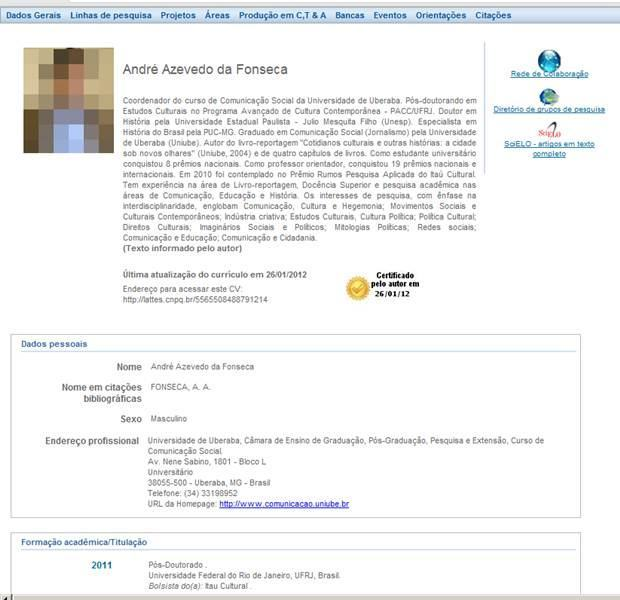
\includegraphics[scale=0.3]{figuras/lattes.jpg}
  \end{figure}
\end{frame}

\begin{frame}{Qualis}
  \begin{figure}
    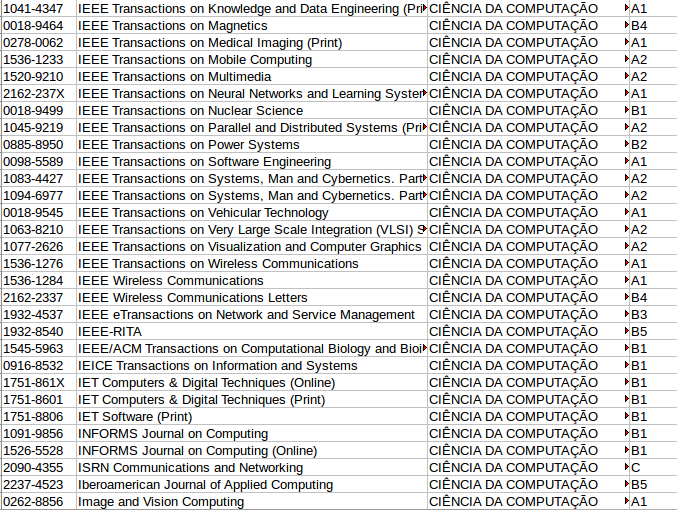
\includegraphics[scale=0.4]{figuras/qualis_exemplo.png}
  \end{figure}
\end{frame}

\begin{frame}
  dsdsa
\end{frame}

\subsection{Objetivos}

\begin{frame}{Objetivos}
  \begin{block}{Objetivo geral}
    Analisar o impacto que o uso de feedback de relevância tem na precisão dos resultados de avaliações realizadas pelo SILQ, efetuado sobre uma nova arquitetura da ferramenta que inclui a criação de API de integração com outros sistemas e a atualização da base de dados conforme as novas classificações Qualis.
  \end{block}
\end{frame}

\begin{frame}{Objetivos específicos}
  \begin{enumerate}[<+->]
    \item Reestruturação da arquitetura e banco de dados do SILQ a fim de suportar classificações de eventos e periódicos disponibilizados em um ritmo anual;

    \item Atualização do banco de dados do sistema com as últimas classificações disponibilizadas pelo Qualis (anos 2013 e 2014);

    \item Criação de uma API pública de disponibilização dos serviços do SILQ, via camada de aplicação REST para integração com outros sistemas;
  \end{enumerate}
\end{frame}

\begin{frame}{Objetivos específicos}
  \begin{enumerate}[<+->]
    \setcounter{enumi}{3}

    \item Alterações na interface do sistema incluindo migração de \textit{framework} de interface, inclusão de controles de \textit{feedback}, novos gráficos de acompanhamento de grupos de pesquisa e melhorias gerais de usabilidade;

    \item Propor novos algoritmos de avaliação baseados em similaridade textual e \textit{feedback} de relevância e verificar se a taxa de acerto do sistema foi melhorada com tal ação.
  \end{enumerate}
\end{frame}

\subsection{Procedimentos metodológicos}

\begin{frame}{Procedimentos metodológicos}
  \begin{enumerate}
    \item Atualização tecnológica e arquitetural
      \begin{itemize}[<2->]
        \item Criação da camada \textit{RESTful};
        \item Migração do \textit{framework} de \textit{interface};
        \item Alteração do modelo lógico p/ suporte aos novos dados Qualis;
      \end{itemize}

    \item Inclusão de \textit{feedback} de relevância
      \begin{itemize}[<3->]
          \item Controles de captação de \textit{feedback};
          \item Desenvolvimento do algoritmo de classificação baseado em \textit{feedback};
          \item Avaliação experimental dos algoritmos.
      \end{itemize}
  \end{enumerate}
\end{frame}

\section{Conceitos}

\begin{frame}{Conceitos}
    Incluir alguns conceitos que sejam interessantes.
    \begin{itemize}
      \item Recuperação de Informação (IR);

      \item \textit{Data-Machting}
      \item query
      \item documentos
      \item SILQ: IR baseado em data matching aproximado
      \item funções de similaridade
      \item valor de similaridade (ou dissimilaridade)
      \item threshold
      \item SILQ: n-grams
      \item como o silq realiza uma avaliação

      \item qual trehsold utilizar? qual função de similaridade utilizar?
      \item Métricas
      \item Precisão e revocação
      \item txa de acerto / exatidão?
      \item conjunto de testes ?
      \item média de rank recíproco

      \item Arquitetura?
    \end{itemize}
\end{frame}

\subsection{Trabalhos correlatos}

\begin{frame}
  TODO: trabalhos correlatos
\end{frame}

\section{Desenvolvimento}

% Slide: trabalhos futuros citados pelo SILQ 1?

\subsection{Alterações tecnológicas}
% Slide: Extração e inserção dos novos dados Qualis
  % Citar que o banco foi alterado
% Slide: Migração tecnológica
  % Criação do Web Service
  % Alterações no Front End
  % Garantia da qualidade: testes de software

\subsection{Uso de feedback de relevância}

\begin{frame}{Obtenção de feedback}
  \begin{figure}
    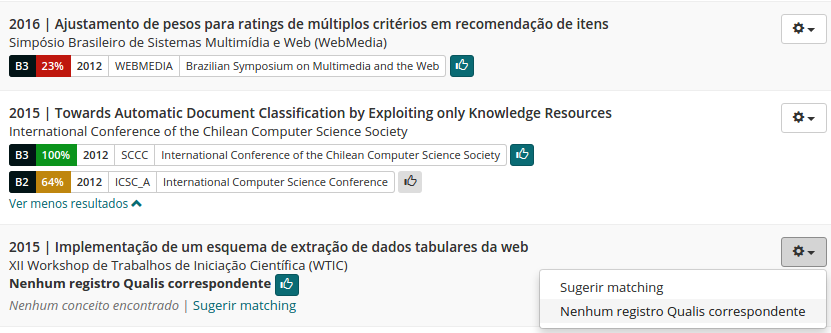
\includegraphics[width=\textwidth]{figuras/feedbacks.png}
    \caption{Controles de feedback da página de resultados de avaliação do SILQ}
  \end{figure}
\end{frame}

% Slide: Obtenção de feedback
% Slide: Algoritmo fb(t)
% Slide: Algoritmo query_aliasing
% Slide: Avaliação experimental

\section{Conclusões}

\begin{frame}{Conclusões}
  Conclusões.
\end{frame}

\begin{frame}{Trabalhos futuros}
  Trabalhos futuros.
\end{frame}

% All of the following is optional and typically not needed.
\appendix
\section<presentation>*{\appendixname}
\subsection<presentation>*{Encerramento}

\begin{frame}
  \begin{center}
    \large Análise do uso de \textit{feedback} de relevância no Sistema de Integração Lattes-Qualis (SILQ)

    \hfill \break

    \LARGE Dúvidas?

    \hfill \break
    \normalsize Carlos Bonetti \\
    \textit{carlosbonetti.mail@gmail.com}
  \end{center}
\end{frame}

\end{document}
